\chapter{Intro/Background/Theory 2} 

\label{Chapter2} 



%-----------------------------------------------------------
\section{Atomic-scale modelling}
%-----------------------------------------------------------
Knowledge of thermal conductivity is important for modelling the deep earth, but can not be measured experimentally at core mantle boundary conditions. Atomic scale simulations sidestep experimental limitations, but system size must be chosen carefully in order to determine accurate conductivity values. Classical molecular dynamics approaches are utilised, with the intention of constraining appropriate system parameters.

A range of atomic scale simulation methods are available to determine the lattice thermal conductivity of materials. These are invaluable for calculating thermal conductivity at conditions of which experiments are difficult, e.g. the extreme conditions found in the Earth's lower mantle (pressures and temperatures up to 136~GPa and 4000~K at the core-mantle boundary). 

%---------------------------------------
\subsection{Molecular dynamics}
%---------------------------------------

%-------------------
\subsubsection{Parameter drift/convergence}
%-------------------
We ensure all calculations are run for a sufficient length of time for the conductivity value to converge. When conductivity fails to converge it means either the simulations needs to be run for longer (unlikely with our nanosecond-scale classical calculations), or the system temperature has drifted. When NVE simulations are run for a long time there is noticable drift in the average system temperature (due to numerical approximations in the equation of motion), which in turn causes drift in the computed conductivity.

NPT-NVT-NVE PROCESS

%---------------------------------------
\subsection{Interatomic potentials / Atomic interactions?}
%---------------------------------------
With the interatomic potential of \citet{Oganov2000} we simulate bridgmanite (MgSiO$_3$ perovskite). To assess finite-size effects we use larger simulation cells than those employed in previous studies. The atom counts associated with these cells (the largest cell considered having over 100,000 atoms) means an ab initio study would be impractical, necessitating the use of interatomic potentials. We expect the potentials to represent the finite size effects well, even if computed conductivities may inaccurate compared to first-principles calculations.

WHY OGANOV? 

WHAT CUTOFFS?

%---------------------------------------
\subsection{LAMMPS}
%---------------------------------------
LAMMPS (Large-scale Atomic/Molecular Massively Parallel Simulator) is a classical molecular dynamics code \citep{Plimpton1995}.

%---------------------------------------
\subsection{DFT/other}
%---------------------------------------
Required? Subsubsection somewhere?



%-----------------------------------------------------------
\section{Computing \tc}
%-----------------------------------------------------------
\citet{Stackhouse2010} review different methods to compute thermal conductivity, in the present work we focus on two of these:
(1) Equilibrium molecular dynamics based on the Green-Kubo relations to determine the thermal conductivity from heat flux fluctuations and their time-dependence \citep{Green1954,Kubo1957,Kubo1966,Schelling2002}. 
(2) The non-equilbrium molecular dynamics-based ``direct method'', where thermal conductivity is calculated from an imposed heat flux and corresponding temperature gradient via Fourier's Law \citep{Muller-Plathe1997,Nieto-Draghi2013}.

%---------------------------------------
\subsection{Finite-size effects}
%---------------------------------------
[[[Give its own section, or as subsection in each method?]]]\\
Computational techniques are not limited by the reproduction of physical conditions like experiments, however they are affected by the size and shape of the simulation cell. The effects of the finite system size available for computation must be checked, as systems with too few atoms are sometimes unable to reproduce the behaviour of the bulk material. If the wavelength of a phonon is too long to fit into a cell, it is not able to transport heat like it should. In the case of the direct method, the length to cross sectional area (CSA) aspect ratio can also matter.

Considering systems of varying size, length-dependent conductivities are obtained from the direct method and extrapolated to the bulk material (\citet{Schelling2002}). The validity of this extrapolation procedure have been called into question (e.g. \citet{Sellan2010}), when a linear trend cannot be fit through the length-dependent conductivities. We describe finite-size effects (FSE) which cause the conductivity result of a simulation to diverge from the value expected by a linear trend, and offer a comparison with results obtained from the Green-Kubo method. The two methods have previously been compared (e.g. \citet{Schelling2002} [[[REFERENCED EARLIER IN THIS PARAGRAPH, THIS OKAY?]]] ), and have been found to give results in good agreement.

The finite-size effects (FSE) I describe are associated with phonon-phonon scattering, or the lack thereof, and boundary-scattering or truncation of phonon mean free path due to limited system sizes. These phenomena combine to misrepresent the phonon behaviour of the bulk material. 

The FSE observed for a material change with thermal conductivity/phonon MFP, and thus are pressure, temperature, and composition sensitive. Higher conductivity(or is it MFP?) materials/conditions require larger systems to eliminate FSE (and vice versa) [[[BUT IS THIS TRUE?]]].



%---------------------------------------
\subsection{Direct method}
%---------------------------------------
The direct method is the computational implementation of a typical experiment to measure thermal conductivity, using Fourier's law to relate heat flux ($q$) and temperature gradient ($\nabla{T}$) to thermal conductivity ($k$), 
\begin{equation}
q=-k \nabla{T} \label{fourier}.
\end{equation}

%-------------------
\subsubsection{System setup}
%-------------------

In the direct method energy is transferred from one group of atoms to another, creating hot and cold regions between which heat flows. The resultant temperature gradient is measured by calculating the temperature of individual groups of atoms along the direction of the heat flux. Simulation cells tend to be long relative to their cross-sectional area, defined as height by width (see Figure~\ref{fig:cell_dia}). Cell boundaries are periodic and the hot and cold sections are half the cell length apart, meaning heat flows in both directions from hot to cold (one of which is across the length-end periodic boundary). This results in two similar temperature gradients which can be averaged.

\begin{figure}[h]
  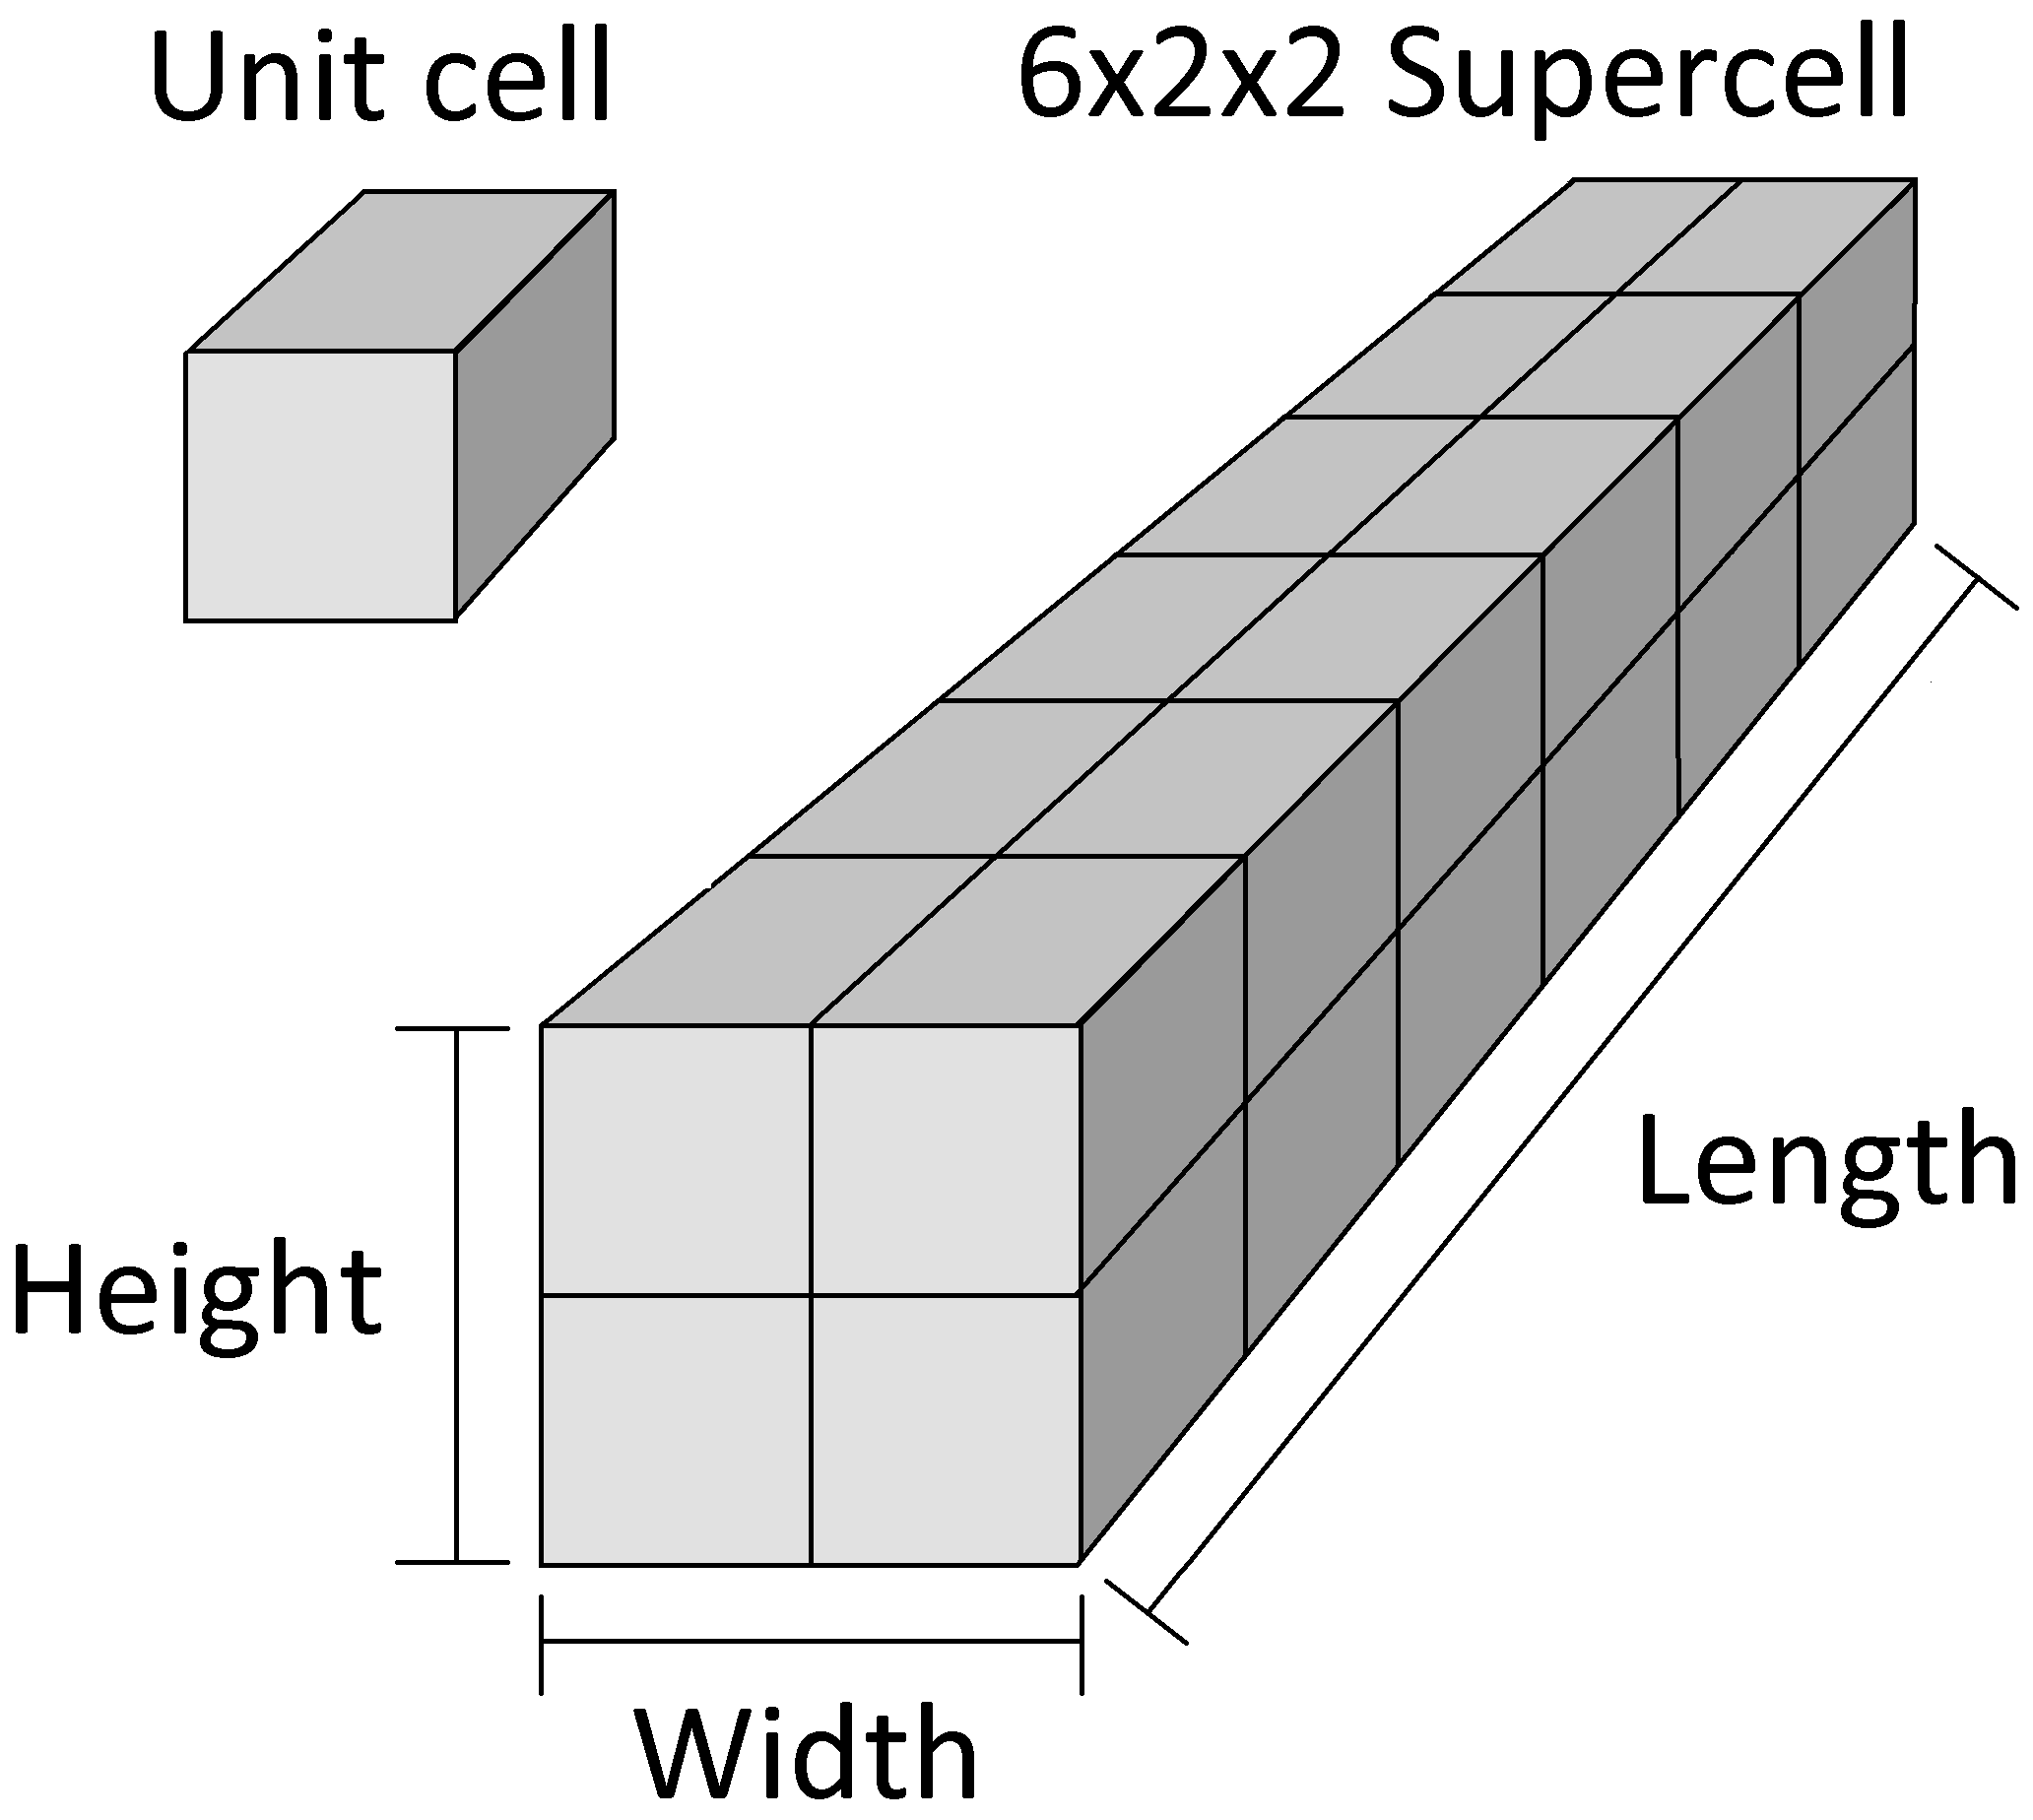
\includegraphics[width=\linewidth]{Figures/cell_diagram.png}
  \caption{The unit cell represents the smallest box of atoms that can be replicated to produce a crystal structure. A supercell is an arrangement of unit cells.}
  \label{fig:cell_dia}
\end{figure}

\begin{figure}[h]
  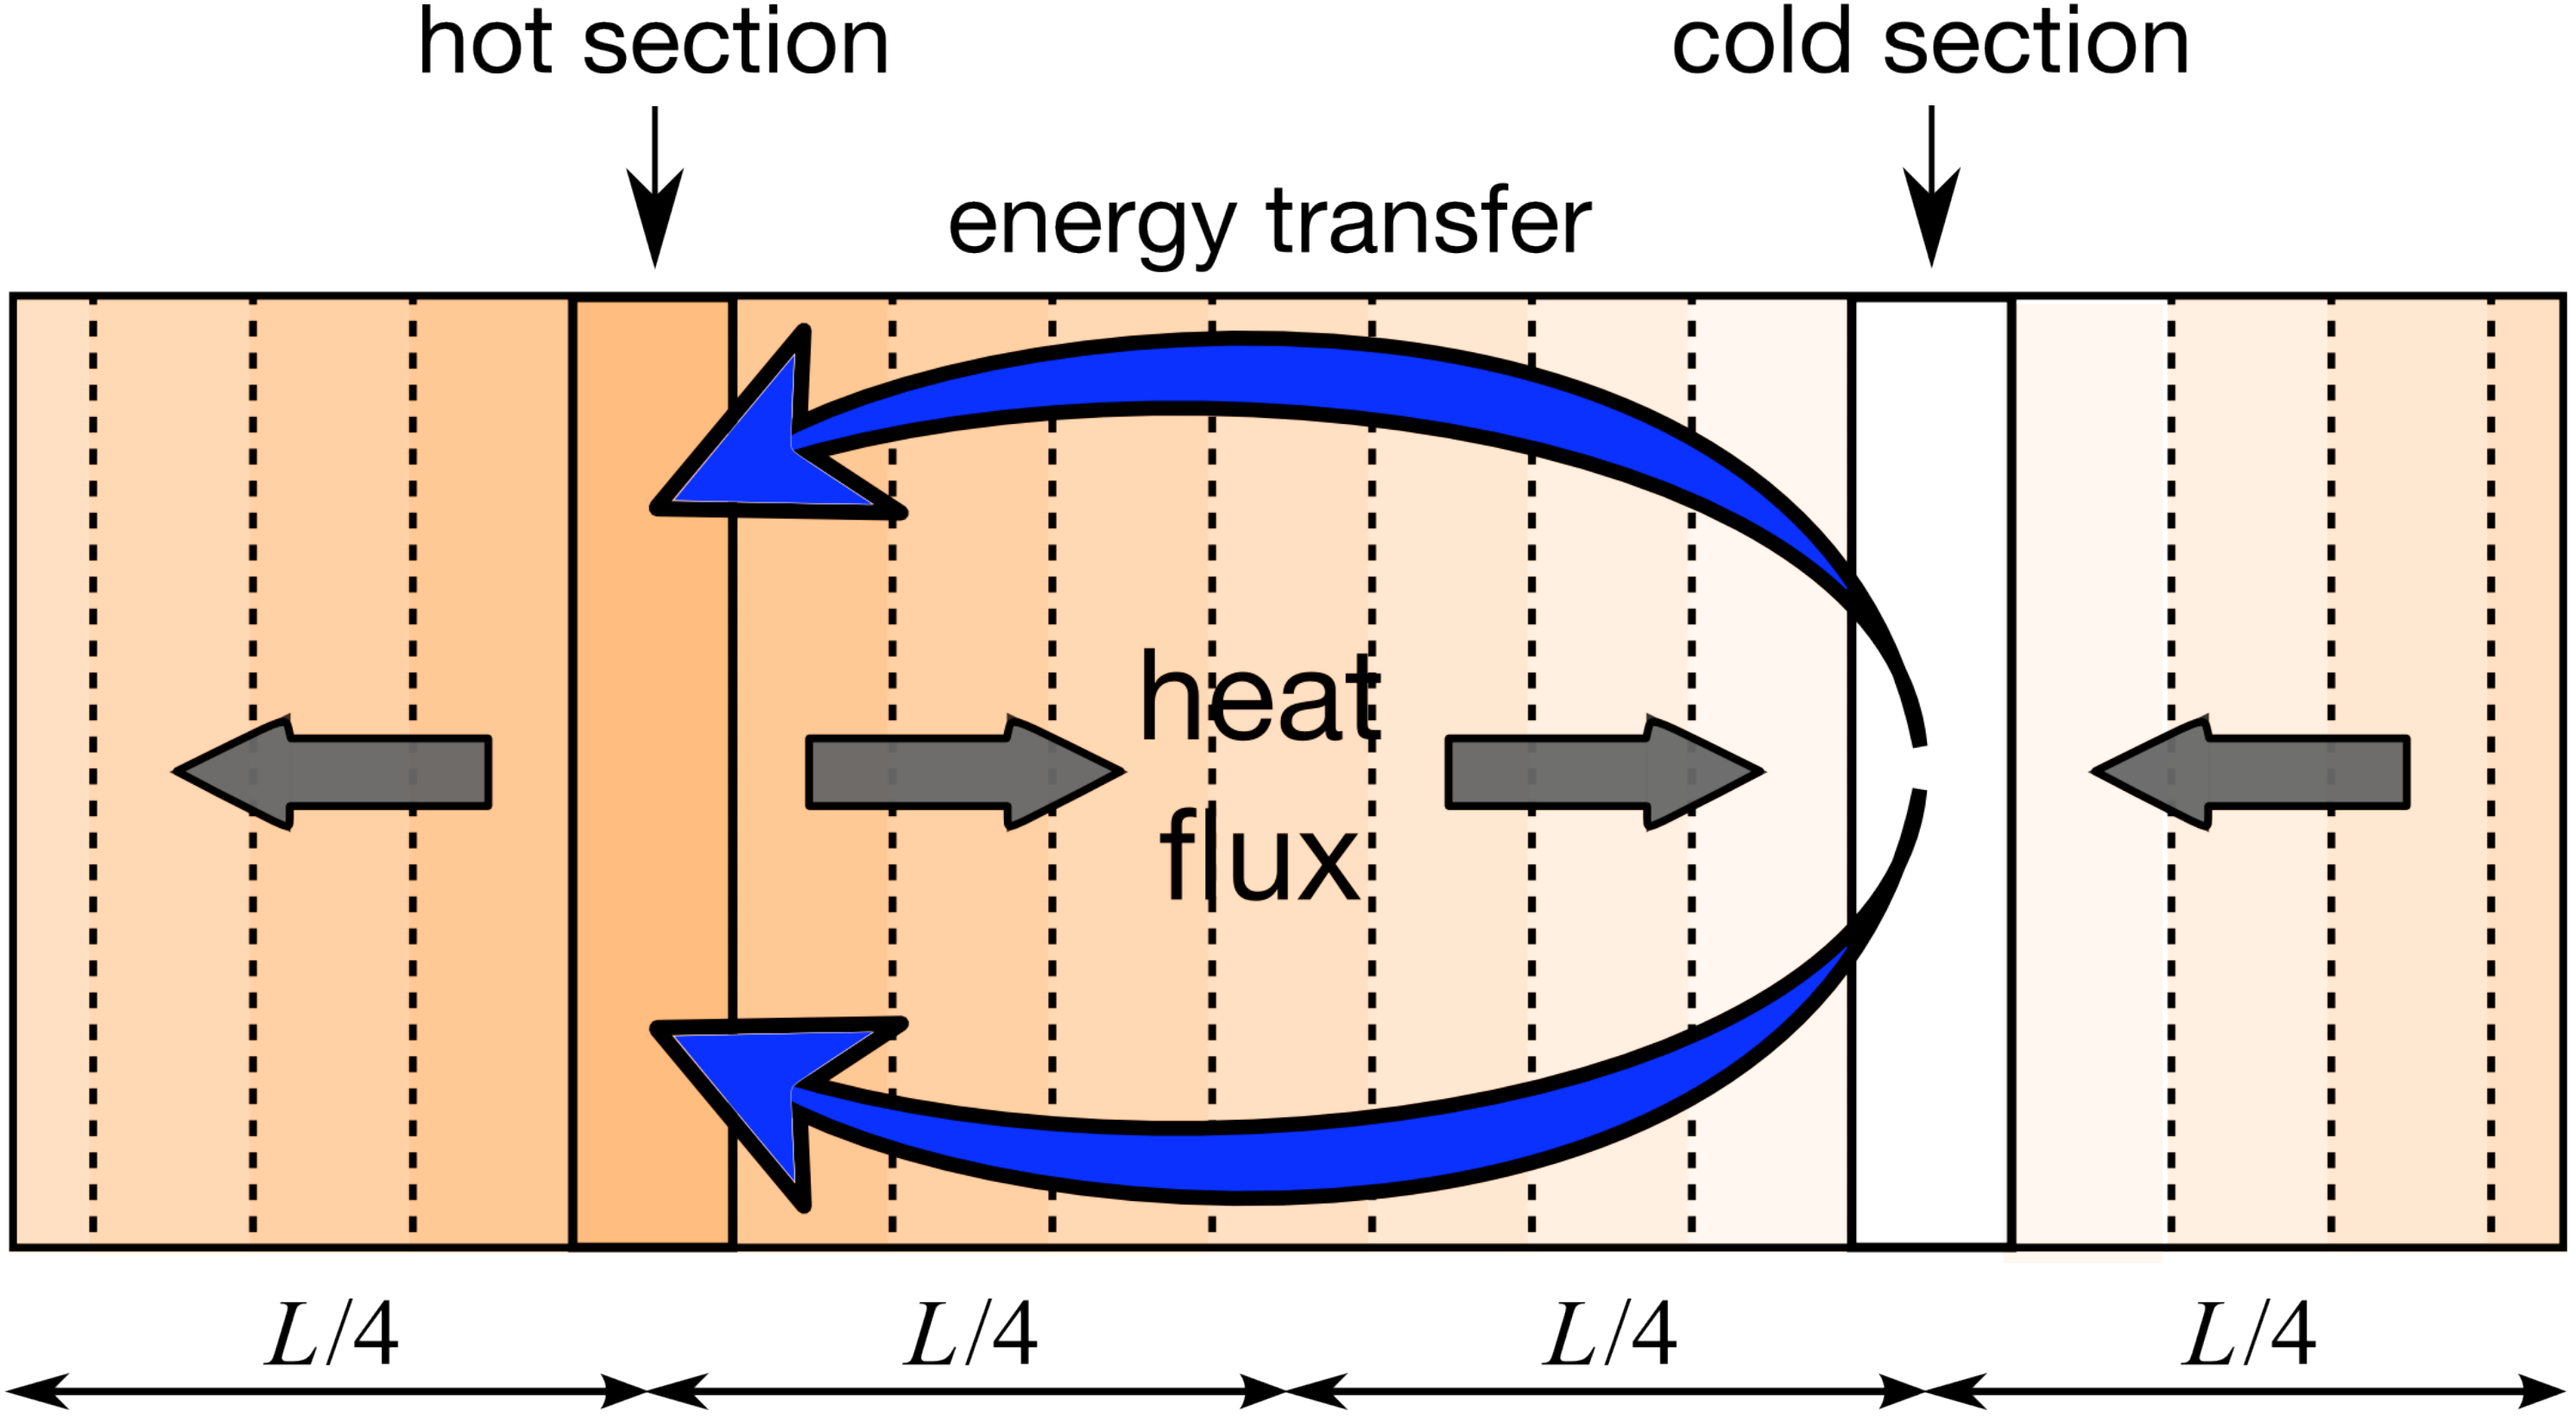
\includegraphics[width=\linewidth]{Figures/ss_direct_mod.png}
  \caption{Movement and distribution of heat in the direct method. Orange to white scale represents temperature \citep[modified from][]{Stackhouse2015}.}
  \label{fig:ss_direct}
\end{figure}

From kinetic theory [[[REF?]]], conductivities computed by the direct method ($k_L$) are dependent on length of simulation cell,
\begin{equation}
k_{L} = \frac{1}{3} C_{V} v l_{L} \label{length-dep},
\end{equation}

where $C_v$ is the volumetric heat capacity, $v$ is the average phonon drift velocity, and $l_L$ is the phonon mean free path. 

%-------------------
\subsubsection{Data processing}
%-------------------

The finite size of the simulation cell truncates the mean free path, underestimating conductivity compared to that of the bulk material ($k_\infty$). Using results from simulations of varying cell length ($L$), conductivity is extrapolated to a length-independent value (where $b$ is a material dependent parameter),

\begin{equation}
{k_{L}}^{-1} = b L^{-1} + {k_{\infty}}^{-1} \label{linear-extrap}.
\end{equation}

Inverse conductivities from direct method simulations are plotted against corresponding inverse cell lengths. A straight line is fit to the data and extrapolated to the y-axis (at which the inverse cell length equals zero and real length equals infinity), where the intercept gives the inverse of the bulk material conductivity \citep{Schelling2002}.

\begin{figure}[h]
  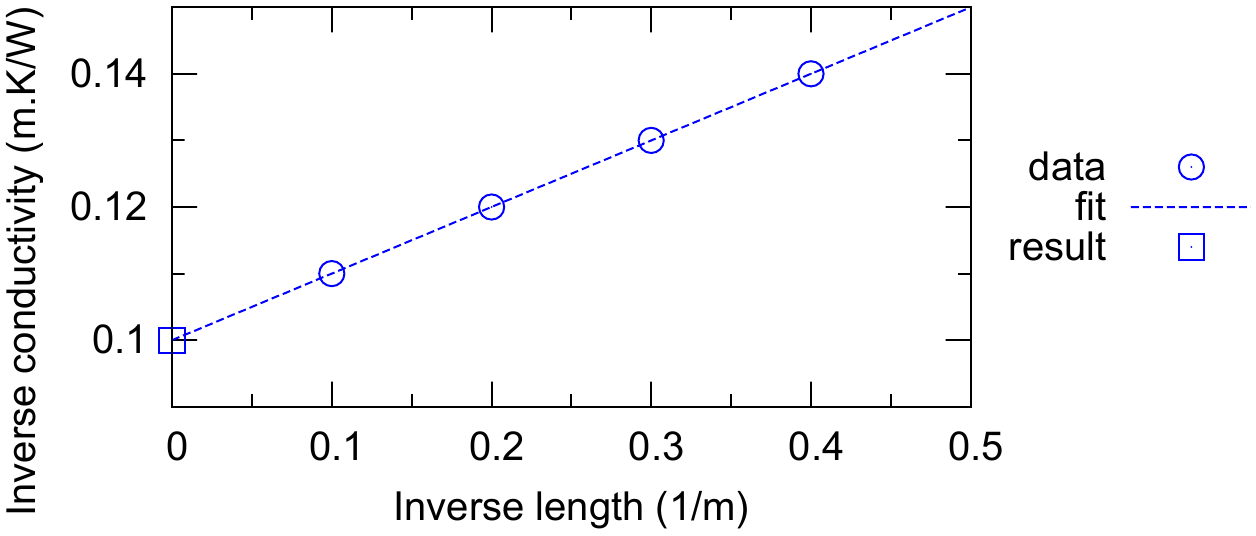
\includegraphics[width=\linewidth]{Figures/ideal_extrap.png}
  \caption{Idealised example of linear extrapolation procedure. Inverse computed conductivities are plotted against inverse simulation lengths. Extrapolation to y-axis gives conductivity of an infinite system length, i.e. the bulk material.}
  \label{fig:ideal}
\end{figure}

%-------------------
\subsubsection{Finite-size effects}
%-------------------

Problems arise when the data do not support a linear trend. There are two effects of finite system size that can cause an individual direct method simulation to diverge away from an inferred/expected linear trend, both of which result in overestimation of the length-dependent conductivity data point. First, when the distance between hot and cold sections (controlled by cell length) is shorter than the MFP, phonons travel ballistically (i.e. without any scattering events) from heat source to sink \citep{Sellan2010}. Conductivites in shorter length cells are overestimated when this occurs, reducing the gradient of the linear fit and thus underestimating the extrapolated conductivity.

For a given length, conductivity is dependent on the CSA, or aspect ratio of the simulation cell. Conductivity is overestimated due to an underestimation of phonon-phonon scattering, from sparse phonon phase sampling in cells where cross-section is small compared to length. Phonons that aren't resolved cannot contribute to phonon-phonon scattering effects. Reduced scattering means heat transport is artificially more efficient than expected from the bulk material. 

[[[SPECIFIC ALERT, REFERENCING THINGS I FOUND]]] However, the required CSA to abate this FSE is length-dependent. When the CSA is smaller than required for all cell lengths (e.g. 1x1 [FIGURE]), all conductivities are overestimated \citep[][albeit for nanotube diameter?]{Thomas2010}. As the CSA is increased, the data points (and thus also the extrapolated result) shift to lower conductivities (higher inverse conductivities). It is at this point that the short cells with lengths of similar order, will report conductivities converged with respect to CSA. Assuming these cells are sufficiently long to avoid the ballistic phonon transport (BPT), a linear fit can be extrapolated to obtain conductivity (for CSA around 2x2, the case at 4000~K). 

The convergence is not necessarily observed concurrently for longer cells however, where they might show overestimated conductivities compared to the fit through the short cells (\cite{Hu2011}). This would cause the fit to all data to be steeper than it should, increasing the extrapolated result.  [[[HOPEFULLY THIS IS TRUE]]] I can show that increasing CSA does not change the computed conductivity at short lengths, but does reduce values from longer cells and bring them into alignment with the expected fit.

%-------------------
\subsubsection{Other NEMD}
%-------------------
Fixed ends?

Sinusoidal temperature perturbation.


%%%MOVE TO 3
%By comparing results with the Green-Kubo method, we will constrain the cell lengths in the linear extrapolation region to mitigate these effects. 
%[[[SPECIFIC ALERT, REFERENCING THINGS I FOUND]]] The effect of FSE on conductivity results depends on the magnitude of conductivity/phonon MFP/physical conditions. At low kappa/low MFP/high T/ (my 4000~K), no BPT is observed, and short cells (>16 unit cells) can be used for extrapolation. In fact, short cells must be used to extrapolate, unless CSA considersations are made to ensure convergence of long cell results.
%[[[SPECIFIC ALERT, REFERENCING THINGS I FOUND]]] At high kappa/high MFP/low T (my 1000~K), BPT must considered at the shorter cells (just 6?). Effectively there is a "sweet-spot", a window of cell lengths for a given CSA that produce consistently-converged results. Long cells outside of the window require a larger CSA, short cells outside show BPT. At 4000~K the lower limit of the window is smaller than the minimum cell length considered, and the upper limit is between 16-24 unit cells. For 1000~K the lower limit of the window moves inside the simulated cell length range around 6-8 unit cells (OR MORE?). The upper limit of the window appears to be larger than 96 unit cells, including all long cells up to this value produces an extrapolation in agreement with GK.
%We have investigated this effect by varying CSA for a range of cell lengths, extrapolated conductivity decreases and eventually converges with CSA. We will use the smallest area that produces the converged conductivity for computational efficiency. 


%---------------------------------------
\subsection{Green-Kubo}
%---------------------------------------
The Green-Kubo method uses auto-correlation functions (ACFs) to quantify time-dependence of heat fluxes (shown in Figure~\ref{fig:gk_acf}, and Equation \ref{acf-j}), in a simulation cell of roughly cubic dimensions (WHY??) and spatially-consistent average temperature. Instantaneous heat fluxes can be used to determine how energy is dissipated within a system, where brief flux events mean heat is transferred quickly indicating high thermal conductivity [[[and vice versa, BUT IS THIS TRUE?]]]. 

\begin{figure}[h]
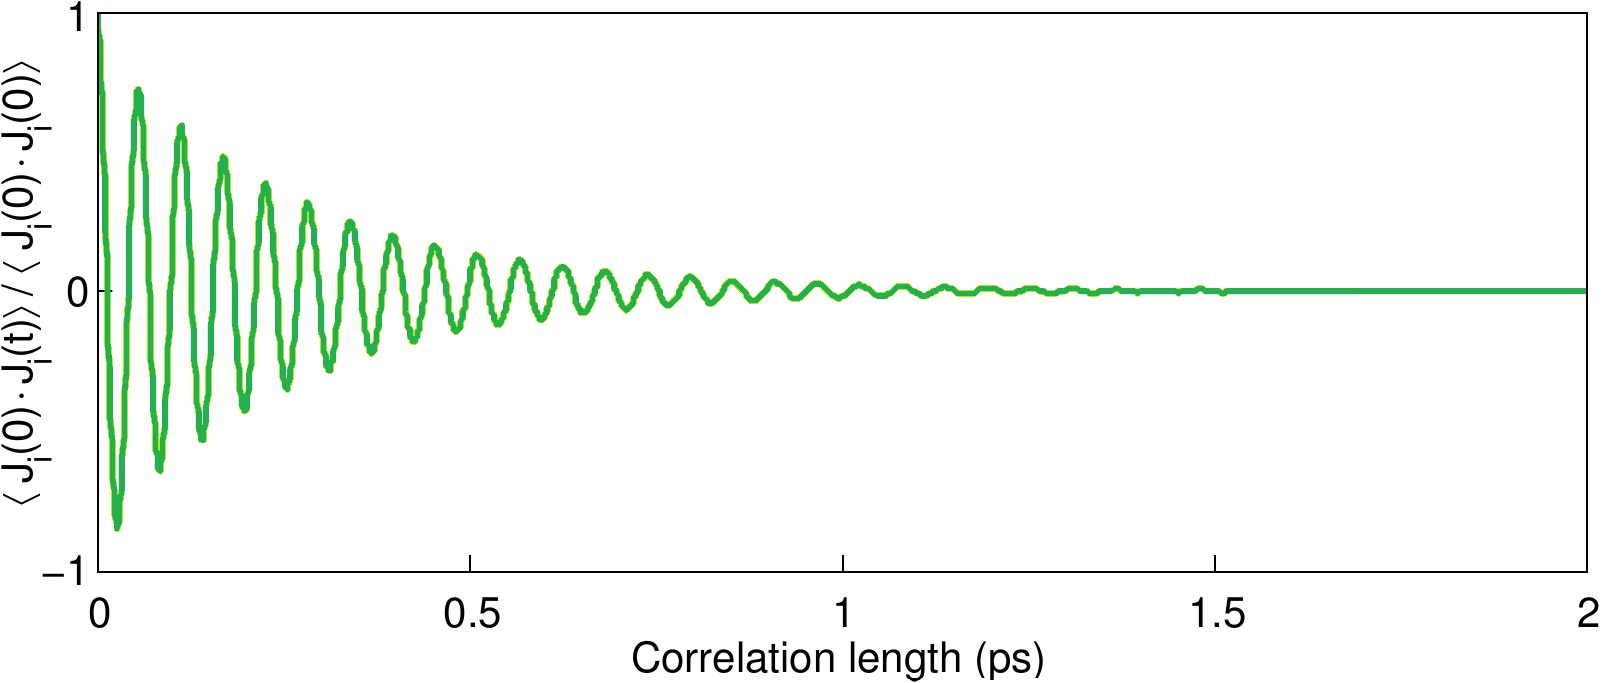
\includegraphics[width=\linewidth]{Figures/gk_acf.png}
\caption{Normalised ACF. Correlation is taken over a longer length than shown on this plot (100 ps), however the function decays to less than 1\% of its initial value at 2~ps. It continues to oscillate about zero, with a positive average value.}
\label{fig:gk_acf}
\end{figure}

The auto-correlation is obtained over the net heat flux series in each crystallographic direction, for a timescale up to a chosen correlation length.
~
\begin{equation}
ACF_i = \left \langle J_i(0) \cdot  J_i(t) \right \rangle,
\label{acf-j}
\end{equation}
~
where $i$ specifies direction, $J$ is heat flux, and $t$ is the correlation length. The integral of heat flux ACF is proportional to thermal conductivity via the Green-Kubo equation (see Figure~\ref{fig:gk_int} and Equation \ref{gk-int}), 
~
\begin{equation}
\kappa_i = \frac{V}{k_{B}T^{2}} \int_{0}^{\infty} \left \langle J_i(0) \cdot  J_i(t) \right \rangle dt ,
\label{gk-int}
\end{equation}
~
[[[I am using ``k''s and ``kappa''s to represent \tc, kappa here and k earlier?]]] where $V$ is the simulation cell volume, $k_B$ is the Boltzmann constant, and $T$ is the average temperature of the system. In this study we use Green-Kubo results as an independent check on the direct method, as they do not have the same finite size-effects. Obtaining a converged conductivity result simply depends on using a large enough cell volume / number of atoms. 

\begin{figure}[h]
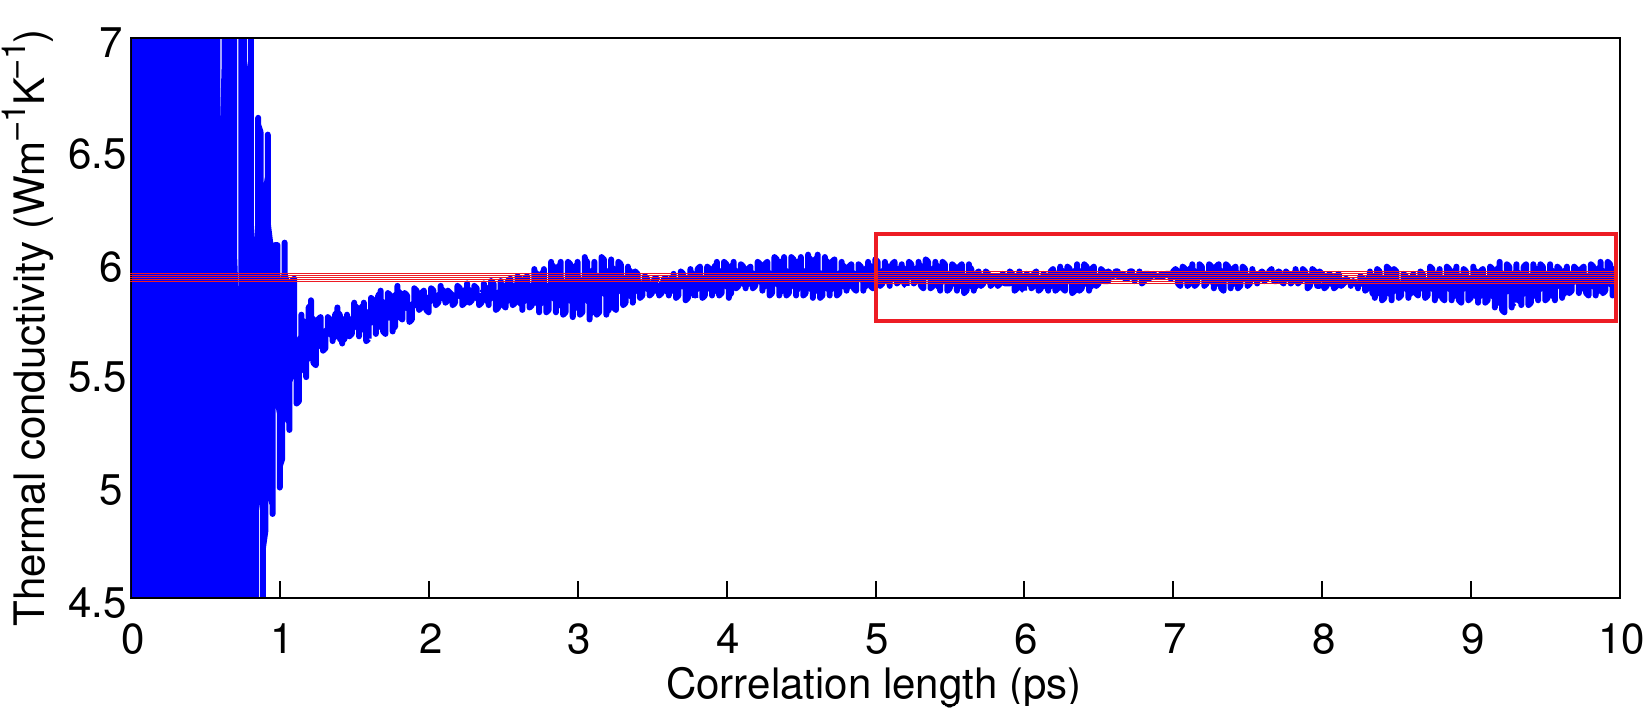
\includegraphics[width=\linewidth]{Figures/gk_int.png}
\caption{Integrated ACF, multiplied by constants to get thermal conductivity. Large variation in the first 1 ps corresponds to the correlation time where the ACF is unconverged (still decaying / large oscillations). Thermal conductivity is averaged from correlation time of 5~ps - 10~ps (region in red box).}
\label{fig:gk_int}
\end{figure}

The individual integrals obtained from the Green-Kubo show variation from the average combined integral on the order of the mean. Many simulations from different intital temperature conditions are required in order to ensure good sampling of conductivity, as well as ensuring the computation time for each is long enough for convergence. This makes Green-Kubo a computationally expensive method, especially for large systems.

The ACF should decay to zero as correlation time tends to infinity, however noise in the ACF prevents this. This will ultimately cause the integral to diverge/drift on long timescales. \citet{Howell2012} fits a series of exponential decays to their ACF, forcing the expected decay to zero and subsequent (constant) integral convergence. This is represents a significant improvement on the conductivity estimate at long correlation lengths, but is mostly similar with the un-fit integrals early in the correlation. (INTEGRAL DRIFT FIGURE, JUST THE ONE INTEGRAL FOR 100PS)

(STACKHOUSE 2010 REFERENCES Volz and Chen 2000; Sun and Murthy 2006)



%---------------------------------------
\subsection{Other}
%---------------------------------------
(3) Anharmonic lattice dynamics \citep{Tang2009}. %(BTE)CHERNATYNSKIY and PHILLPOT 2010?
\\
(4) Combined quasiharmonic lattice dynamics and molecular dynamics method \citep{DeKoker2009}.



%-----------------------------------------------------------
\section{Previous work}
%-----------------------------------------------------------

%---------------------------------------
\subsection{Method comparison}
%---------------------------------------

%---------------------------------------
\subsection{Finite-size effects}
%---------------------------------------
Should this section be interspersed into when FSE are mentioned in methods?

%-------------------
\subsubsection{STUFF THAT MIGHT BE WRONG BECAUSE FSE?}
%-------------------


